% Part: sets-functions-relations
% Chapter: arithmetization
% Section:reals

\documentclass[../../../include/open-logic-section]{subfiles}

\begin{document}

\olfileid[ar]{sfr}{arith}{real}
\olsection{المستقيم الحقيقي}

وننتقل الآن إلى بناء الأعداد الحقيقية من النسبية. غير أن هذا البناء يقتضي أن نبين أولًا ما \emph{تنفرد به} الحقيقية عن النسبية.

كثير من أحكام الأعداد الحقيقية يجري على نحو أحكام النسبية؛ فكلتاهما، بالاصطلاح التقني، \emph{حقل مرتب} (وتعريفه في \olref[check]{orderedfield}). ومن أتم تمارين \olref[sfr][siz][]{chap} علم أن الحقيقية أكثر عددًا من النسبية على وجه الصرامة، أي $\cardless{\Rat}{\Real}$؛ وأول من أثبت ذلك كانتور. أما وجود غير النسبية---وهي أعداد حقيقية ليست نسبية---فمعروف منذ نحو ألفين وخمسمئة سنة. ومن شواهده:
%\footnote{Now: ``$\sqrt{2}$'' equally refers to both the positive and the negative roots; but in the next few pages, I'll forget about this, and consider only the positive root.}
\begin{thm}\ollabel{root2irrational}
$\sqrt{{\OLMathNumeral{2}}}$ غير نسبي؛ أي $\sqrt{{\OLMathNumeral{2}}} \notin \Rat$
\end{thm}

\begin{proof}
% تصحيح برهاني (0044-I1): اختير تمثيل أصغر في مجموع البسط والمقام، وهو ما تحتاج إليه حجتا النزول التاليتان.
لنفرض، طلبًا للخلف، أن $\sqrt{{\OLMathNumeral{2}}}$ نسبي. فيكون $\sqrt{{\OLMathNumeral{2}}} =
\nicefrac{{\OLId{latin-ordinary}{m}}}{{\OLId{latin-ordinary}{n}}}$ لعددين طبيعيين موجبين ${\OLId{latin-ordinary}{m}}$ و${\OLId{latin-ordinary}{n}}$. ونختارهما بحيث يكون
${\OLId{latin-ordinary}{m}}+{\OLId{latin-ordinary}{n}}$ أصغر ما يمكن بين جميع هذه التمثيلات. ومن المساواة ينتج
${\OLId{latin-ordinary}{m}}^{{\OLMathNumeral{2}}} = {\OLMathNumeral{2}}{\OLId{latin-ordinary}{n}}^{{\OLMathNumeral{2}}}$. ثم لنا في إتمام البرهان وجهان.

\emph{الوجه الأول هندسي}، وهو لتننباوم.\footnote{نقل هذا البرهان في \cite{Conway2006}.} انظر إلى المربعات في الرسم:
\begin{center}
	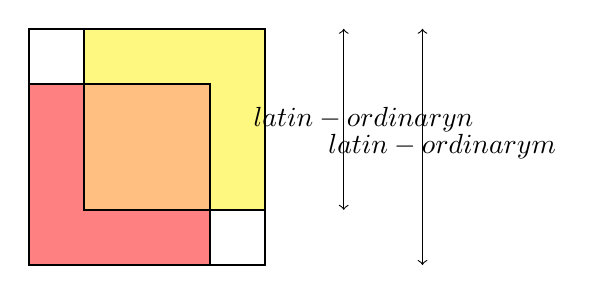
\begin{tikzpicture}
		\draw[thick] (0,0) rectangle (3,3);
		\draw[thick, fill=red!50] (0,0) rectangle (2.3,2.3);
		\draw[thick, fill=yellow!50] (0.7,0.7) rectangle (3, 3);
		\draw[thick, fill=orange!50] (0.7,0.7) rectangle (2.3, 2.3);
		\draw[<->] (4, 0.7)--(4, 3);
		\node at (4.25, 1.85) (n) {${\OLId{latin-ordinary}{n}}$};
		\draw[<->] (5, 0)--(5, 3);
		\node at (5.25, 1.5) (m) {${\OLId{latin-ordinary}{m}}$};
	\end{tikzpicture}
\end{center}
لما كان ${\OLId{latin-ordinary}{m}}^{\OLMathNumeral{2}} = {\OLMathNumeral{2}}{\OLId{latin-ordinary}{n}}^{\OLMathNumeral{2}}$، ساوت مساحة تداخل المربعين ذوي الضلع ${\OLId{latin-ordinary}{n}}$ مساحة ما لم يغطياه من المربع الكبير. فمساحة المربع البرتقالي تساوي مجموع مساحتي المربعين غير المظللين. فإذا سمينا ضلع البرتقالي ${\OLId{latin-ordinary}{p}}$ وضلع كل غير مظلل ${\OLId{latin-ordinary}{q}}$، حصل ${\OLId{latin-ordinary}{p}}^{\OLMathNumeral{2}} = {\OLMathNumeral{2}}{\OLId{latin-ordinary}{q}}^{\OLMathNumeral{2}}$. فيكون $\sqrt{{\OLMathNumeral{2}}} = \nicefrac{{\OLId{latin-ordinary}{p}}}{{\OLId{latin-ordinary}{q}}}$، مع ${\OLId{latin-ordinary}{p}} < {\OLId{latin-ordinary}{m}}$ و${\OLId{latin-ordinary}{q}} < {\OLId{latin-ordinary}{n}}$ و${\OLId{latin-ordinary}{p}}, {\OLId{latin-ordinary}{q}} \in
\Nat$. وهذا يناقض اختيار ${\OLId{latin-ordinary}{m}}$ و${\OLId{latin-ordinary}{n}}$ أصغر ما يمكن.

\emph{الوجه الثاني صوري.} من ${\OLId{latin-ordinary}{m}}^{{\OLMathNumeral{2}}} = {\OLMathNumeral{2}}{\OLId{latin-ordinary}{n}}^{{\OLMathNumeral{2}}}$ يلزم أن ${\OLId{latin-ordinary}{m}}$ زوجي؛ إذ لو كان ${\OLId{latin-ordinary}{x}}$ فرديًّا لكان ${\OLId{latin-ordinary}{x}}^{\OLMathNumeral{2}}$ فرديًّا، وإثباته يسير. فنكتب ${\OLId{latin-ordinary}{m}} = {\OLMathNumeral{2}}{\OLId{latin-ordinary}{r}}$ لبعض ${\OLId{latin-ordinary}{r}} \in \Nat$، وبالتعويض والحذف نحصل على ${\OLMathNumeral{2}}{\OLId{latin-ordinary}{r}}^{\OLMathNumeral{2}} = {\OLId{latin-ordinary}{n}}^{\OLMathNumeral{2}}$،
		%				\begin{align*}
		%					(2q)^{2} &= 2n^{2}\\
		%					4q^{2} &= 2n^{2}\\
		%					2q^{2} &= n^{2}
		%				\end{align*}
فيكون ${\OLId{latin-ordinary}{n}}$ زوجيًّا أيضًا؛ فلنكتب~${\OLId{latin-ordinary}{n}}={\OLMathNumeral{2}}{\OLId{latin-ordinary}{s}}$. فينتج
$\sqrt{{\OLMathNumeral{2}}}=\nicefrac{{\OLId{latin-ordinary}{r}}}{{\OLId{latin-ordinary}{s}}}$ مع~${\OLId{latin-ordinary}{r}}+{\OLId{latin-ordinary}{s}}<{\OLId{latin-ordinary}{m}}+{\OLId{latin-ordinary}{n}}$، خلاف اختيار~${\OLId{latin-ordinary}{m}}+{\OLId{latin-ordinary}{n}}$ أصغر ما يمكن.
\end{proof}

وفي هذا البرهان بالرسم مناسبة للرجوع إلى ما في \olref[his][set][mythology]{sec}. فإن تننباوم (\OLClassicalDigits{1927}--\OLClassicalDigits{2006}) من الرياضيين المحدثين، ومع ذلك يجمع برهانه جمالًا لا ينكر، وصرامة تامة، واحتكامًا إلى الحدس الهندسي.

فالأعداد الحقيقية، على كل حال، «أوسع» من النسبية؛ وكأن في النسبية «فجوات» تسدها الحقيقية. وقد أدرك فايرشتراس أن هذا الوصف يرجع إلى خاصية واحدة تميز الحقيقية، وهي خاصية الاكتمال: \emph{كل مجموعة غير خالية من الأعداد الحقيقية، إذا كان لها حد علوي، فلها أصغر حد علوي.}

ويتضح فقدان النسبية لهذه الخاصية إذا أخذنا الأعداد النسبية الأصغر من $\sqrt{{\OLMathNumeral{2}}}$، أي المجموعة
\[
	\Setabs{{\OLId{latin-ordinary}{p}} \in \Rat}{{\OLId{latin-ordinary}{p}}^{\OLMathNumeral{2}} < {\OLMathNumeral{2}} \text{ أو }{\OLId{latin-ordinary}{p}} < {\OLMathNumeral{0}}}
\]
فلها حد علوي نسبي؛ إذ !!{element}s< كلها أصغر من ${\OLMathNumeral{3}}$، مثلًا. وأما أصغر حد علوي لها فقد نتبادر إلى تسميته «$\sqrt{{\OLMathNumeral{2}}}$»؛ لكن قد ثبت أن $\sqrt{{\OLMathNumeral{2}}}$ \emph{ليس} نسبيًّا، ولا يوجد عدد نسبي \emph{أصغر} من سائر الأعداد النسبية التي تزيد على $\sqrt{{\OLMathNumeral{2}}}$. فللمجموعة حد علوي، وليس لها في النسبية أصغر حد علوي؛ ولذلك لا تتمتع الأعداد النسبية بخاصية الاكتمال.

أما المتصل العددي فمقتضى تصوره أن تكون له خاصية الاكتمال. وليس غرضنا الاقتصار على جعل $\sqrt{{\OLMathNumeral{2}}}$ عددًا حقيقيًّا؛ بل الغرض سد جميع «فجوات» المستقيم النسبي، وألا تبقى في المتصل نفسه «فجوة». وهذا ما يكفله لنا الاكتمال.

\end{document}
